\subsection{问题二的模型建立与求解}

\subsubsection{单次检测后的源位置可行域}

记第一检测点为 $S_1$，其对某全向干扰源测得的示向度为 $\theta_1$，相应误差角区为 $C_1$。题设给出目标圆形区域半径为 $1800\ \mathrm{m}$，全向干扰源的实际有效接收半径 $R_s$ 满足
\begin{equation}
  R_s\in[R_{\min},R_{\max}]=[1000,1500]\ \mathrm{m}.
\end{equation}

因为 $S_1$ 已获得示向度，真实源位置 $X$ 必满足 $\|X-S_1\|_2\leq R_s\leq R_{\max}$。因此，式~\eqref{eq:q1-physical-region} 在单次观测下具体化为
\begin{equation}
  K_1=C_1\cap\overline B(O_0,1800)
  \cap\overline B(S_1,R_{\max}).
  \label{eq:q2-physical-region}
\end{equation}

为处理式~\eqref{eq:q2-physical-region} 中的圆弧边界，构造包含原圆盘的固定粗外包。对以 $A$ 为圆心、$R$ 为半径的圆盘，取 $N$ 个等分单位法向量
\begin{equation}
  n_k=\left(\cos\frac{2k\pi}{N},
  \sin\frac{2k\pi}{N}\right)^{\mathsf T},
  \qquad k=0,1,\ldots,N-1,
\end{equation}

并以相应切线半平面之交构造外切正多边形
\begin{equation}
  \widehat B_{\mathrm{out}}^{(N)}(A,R)
  =\bigcap_{k=0}^{N-1}
  \left\{Y:n_k^{\mathsf T}(Y-A)\leq R\right\}.
  \label{eq:q2-outer-polygon}
\end{equation}

本文采用当前程序的固定粗外包构造。取 $N=24$，将目标圆盘和接收上界圆盘分别替换为式~\eqref{eq:q2-outer-polygon} 的外切正多边形，再加入角区 $C_1$ 的两个半平面约束。将这些半平面记为 $\mathcal H_N$，其交集即为后续计算使用的源位置区域：
\begin{equation}
  \widehat K_1=C_1
  \cap\widehat B_{\mathrm{out}}^{(N)}(O_0,1800)
  \cap\widehat B_{\mathrm{out}}^{(N)}(S_1,R_{\max})
  =\bigcap_{H\in\mathcal H_N}H.
  \label{eq:q2-source-region}
\end{equation}

圆盘与固定外切正多边形的几何关系如图~\ref{fig:q2-k1-outer-approx} 所示。正多边形的每条边均与圆相切，因此圆盘完全包含在多边形内；多边形顶点方向处的径向外扩最大。

\begin{figure}[H]
  \centering
  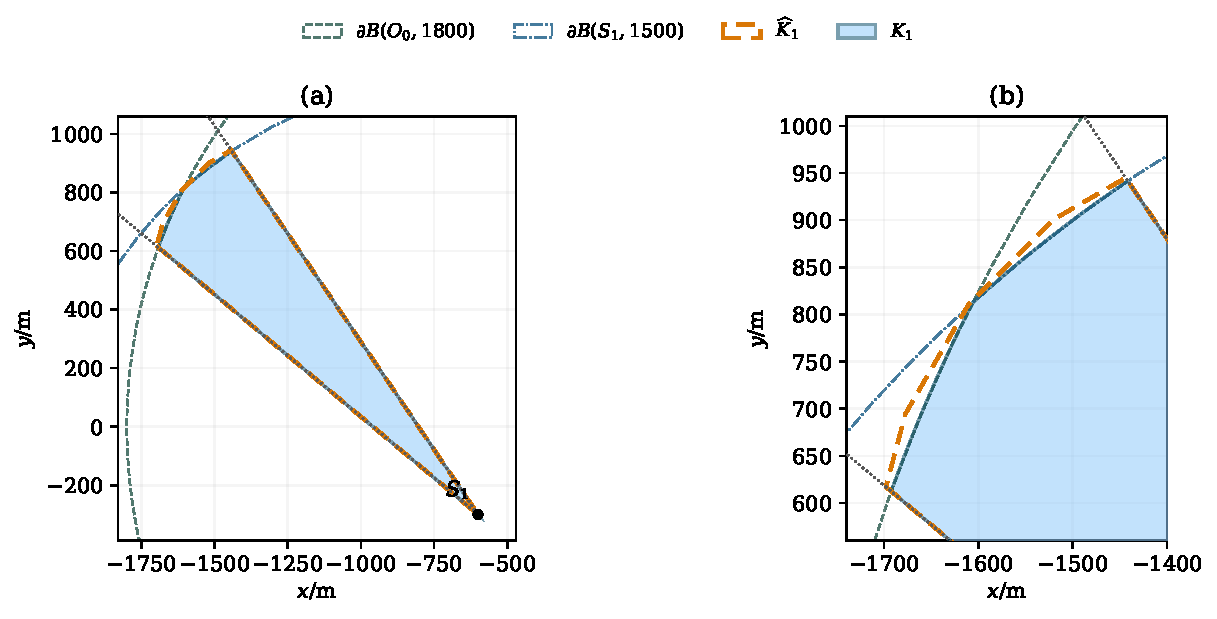
\includegraphics[width=0.64\textwidth]{figures/q2-k1-outer-approx.pdf}
  \caption{外切正多边形局部示意：$T_-,T_+$ 为切点，$V$ 为切线交点，$\Delta_{\mathrm{out}}$ 为最大径向外扩（角度放大，计算取 $N=24$）}
  \label{fig:q2-k1-outer-approx}
\end{figure}

每个切线半平面都包含原圆盘，且角区约束不变，故 $K_1\subseteq\widehat K_1$。这一外近似避免误删真实源，并将圆弧约束转为可求交、枚举顶点及检查覆盖的线性半平面约束。

当 $N=24$ 时，固定粗外包的最大径向外扩量为
\begin{equation}
  \Delta_{\mathrm{out}}(R,N)
  =R\left(\sec\frac{\pi}{N}-1\right).
\end{equation}

半径为 $1800\ \mathrm{m}$ 和 $1500\ \mathrm{m}$ 的圆形区域对应值分别约为 $15.532\ \mathrm{m}$ 和 $12.943\ \mathrm{m}$。这是固定 $24$ 边粗外包的最大径向误差，全部计算均保持这一外包形式。程序中将理论示向度误差 $1^\circ$ 扩大为 $1.005^\circ$，用于降低边界浮点误差导致真实源被错误排除的风险。本文后续模型均沿用这一固定粗外包口径。

\subsubsection{定位不确定性半径}

问题一已证明，以区域直径端点作直径圆时，该圆不一定覆盖整个定位区域。故问题二统一采用最小包围圆尺度描述定位不确定性。对任意非空有界集合 $A$，定义其定位不确定性半径为
\begin{equation}
  \rho(A)=\min_{Q\in\mathbb R^2}
  \max_{Y\in A}\|Y-Q\|_2.
  \label{eq:q2-mec-radius}
\end{equation}

由区域内任意直径端点都必须同时被包围圆覆盖，有
\begin{equation}
  \rho(A)\geq\frac{\operatorname{diam}(A)}{2}.
  \label{eq:q2-diameter-mec}
\end{equation}

直径圆能够覆盖区域时取等号，否则最小包围圆半径更大。记第一次观测后的不确定性半径为 $R_0=\rho(\widehat K_1)$。

设 $\widehat K_1=\operatorname{conv}\{V_1,\ldots,V_m\}$。由问题一的圆覆盖判据，只需对顶点求最小包围圆。遍历单点退化圆、两点直径圆与三个不共线点的外接圆，保留满足
\begin{equation}
  \max_{1\leq l\leq m}\|V_l-Q\|_2\leq r+\tau
  \label{eq:q2-mec-cover-test}
\end{equation}

的候选圆 $(Q,r)$，再取半径最小者；$\tau$ 为数值容差。三点组合有 $O(m^3)$ 个，每圆检查 $m$ 个顶点，故最坏时间复杂度为 $O(m^4)$，适用于本题较少的顶点数。

\subsubsection{第二检测点的候选区域}

若要求无论真实源位于当前可行域中何处、其有效接收半径在题设区间中取何值，第二测点 $s$ 都能收到信号，则必须有
\begin{equation}
  \mathcal F_g(\widehat K_1)
  =\left\{s:\max_{X\in\widehat K_1}
  \|s-X\|_2\leq R_{\min}\right\}.
  \label{eq:q2-guaranteed-region}
\end{equation}

由问题一的圆覆盖判据，一个以 $s$ 为圆心、半径为 $R_{\min}$ 的圆覆盖全部顶点，就覆盖整个 $\widehat K_1$，因此
\begin{equation}
  \mathcal F_g(\widehat K_1)
  =\bigcap_{j=1}^{m}\overline B(V_j,R_{\min}).
  \label{eq:q2-guaranteed-vertices}
\end{equation}

以各 $V_j$ 为圆心构造半径 $R_{\min}$ 的内接正 $72$ 边形，逐一求交得到保证接收域 $\widehat{\mathcal F}_g$。为使输出测点确实可行，此处采用与源区域相反的内近似方向，满足

\begin{equation}
  \widehat{\mathcal F}_g
  \subseteq\mathcal F_g(\widehat K_1)
  \subseteq\mathcal F_g(K_1).
  \label{eq:q2-guaranteed-inclusion}
\end{equation}

其最大径向收缩量为
\begin{equation}
  R_{\min}\left(1-\cos\frac{\pi}{72}\right)
  \approx0.952\ \mathrm{m}.
\end{equation}

故落在 $\widehat{\mathcal F}_g$ 中的测点对当前全向距离接收模型具有保守的接收保证。若 $\widehat{\mathcal F}_g$ 为空，只说明当前内近似未能给出可认证的保证接收点，不由此断言理论保证域必然为空。

另一方面，若只要求存在某个相容源位置使测点可能收到信号，则计算可能接收域
\begin{equation}
  \mathcal F_p
  =\left\{s:\operatorname{dist}(s,\widehat K_1)
  \leq R_{\max}\right\}
  =\widehat K_1\oplus\overline B(O_0,R_{\max}),
  \label{eq:q2-possible-region}
\end{equation}

其中 $\oplus$ 表示 Minkowski 和，即将源区域向外扩张 $R_{\max}$。沿 $72$ 个支撑方向建立半平面可得其外近似 $\widehat{\mathcal F}_p$，用于辅助展示可能接收范围。题目所求第二检测点的候选区域取保证接收域 $\widehat{\mathcal F}_g$，三类区域的关系见图~\ref{fig:q2-reception-regions}。

\begin{figure}[H]
  \centering
  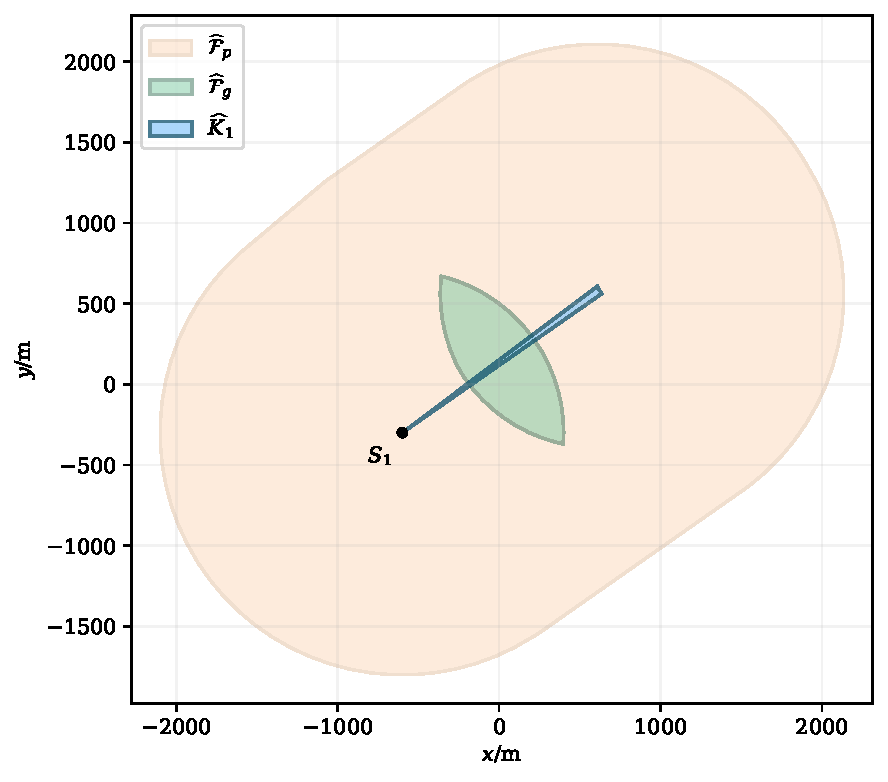
\includegraphics[width=0.68\textwidth]{figures/q2-reception-regions.pdf}
  \caption{源位置区域 $\widehat K_1$、保证接收域 $\widehat{\mathcal F}_g$ 与可能接收域 $\widehat{\mathcal F}_p$ 的关系}
  \label{fig:q2-reception-regions}
\end{figure}

\subsubsection{二次定位不确定性半径的场景预测与行动时间}

选点时尚未获得第二次检测结果，因此通过有限源位置和示向误差场景，预测候选点对定位区域的收缩效果。

记 $\widehat K_1$ 为仅利用第一次检测和物理边界得到的源位置区域，首先离散化干扰源的可能位置。设 $\widehat K_1$ 的顶点按边界顺序为 $V_1,\ldots,V_m$，并令 $V_{m+1}=V_1$。构造三类原始场景：$m$ 个顶点 $V_i$、$m$ 个边中点 $M_i=(V_i+V_{i+1})/2$，以及一个顶点均值中心 $G=m^{-1}\sum_iV_i$，共 $2m+1$ 个点。若其总数不超过 $8$，则全部保留；否则按照固定顺序
\begin{equation}
  V_1,M_1,V_2,M_2,\ldots,V_m,M_m,G
\end{equation}

在序列中等间隔选取 $8$ 个索引，得到有限源位置场景集 $\mathcal S_A$。图~\ref{fig:q2-source-scenarios} 以五边形为例展示了三类原始点及最终保留的 $8$ 个选点。

\begin{figure}[H]
  \centering
  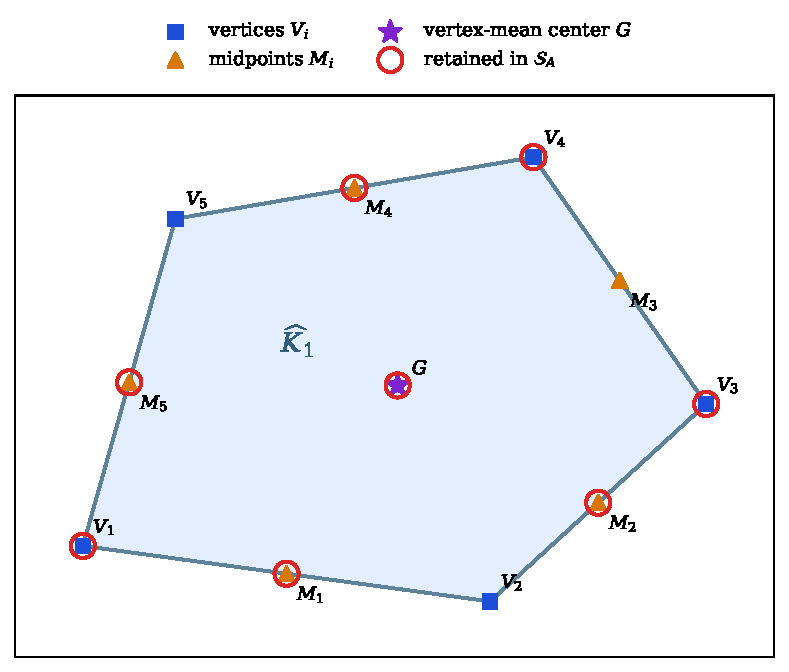
\includegraphics[width=0.66\textwidth]{figures/q2-source-scenarios.pdf}
  \caption{有限源位置场景的构造示例（红色空心圆表示由三类原始点确定性下采样后保留的场景）}
  \label{fig:q2-source-scenarios}
\end{figure}

其次讨论二次检测误差。对假定源位置 $X\in\mathcal S_A$ 和候选检测点 $s$，将在该场景中从 $s$ 指向 $X$ 的无误差方位角记为 $\theta(s,X)$，取有限误差场景集
\begin{equation}
  \mathcal E=\{-\varepsilon,0,+\varepsilon\},
  \qquad \varepsilon=1.005^\circ
\end{equation}

对于 $e\in\mathcal E$，相应的假想二次示向度为
\begin{equation}
  \widehat\theta_2(s;X,e)=\theta(s,X)+e.
\end{equation}

当 $5<\|s-X\|_2\leq R_{\max}$ 且假想示向度有效时，可以得到新的误差角区。因此，该场景对应的预测更新区域为
\begin{equation}
  \widehat K_2(s;X,e)
  =\widehat K_1
  \cap\widehat B_{\mathrm{out}}^{(N)}(s,R_{\max})
  \cap C\bigl(s,\widehat\theta_2(s;X,e),\varepsilon\bigr),
  \label{eq:q2-posterior-region}
\end{equation}

其中 $C(s,\theta,\varepsilon)$ 表示以 $s$ 为顶点、方向为 $\theta$、左右误差界为 $\varepsilon$ 的角区；新增接收圆形区域仍采用第~5.2.1 节相同的固定 $N=24$ 边外切正多边形，全部约束均保持固定粗外包形式。此时 $\rho(\widehat K_2)$ 即为该场景下预测的二次定位不确定性半径。

当 $\|s-X\|_2\leq5\ \mathrm{m}$ 时，题设规定测向机可能返回近距离结果而不给出示向度，此时以 $\min\{5,R_0\}$ 作为定位不确定性半径的保守上界，其中 $R_0=\rho(\widehat K_1)$。综合近距离与有效示向度两类假想结果，定义二次定位不确定性半径的单场景预测值为
\begin{equation}
  r_2(s;X,e)=
  \begin{cases}
    \min\{5,R_0\}, & \|s-X\|_2\leq5,\\
    \rho\bigl(\widehat K_2(s;X,e)\bigr),
      & 5<\|s-X\|_2\leq R_{\max}.
  \end{cases}
\end{equation}

若 $s\notin\mathcal F_g(\widehat K_1)$，则由于真实源位置及其实际接收半径未知，第二次检测还可能返回无信号。当前模型不利用无信号结果进一步排除位置，而保守地认为定位区域未发生收缩，将该分支的定位不确定性半径预测值记为 $R_0$。计算时通过 $\widehat K_1$ 的顶点最大距离检验式~\eqref{eq:q2-guaranteed-region} 的保证接收条件。由此定义二次定位不确定性半径的有限场景最坏预测值
\begin{equation}
  R_{\mathrm{wc}}(s)
  =\max\left(
  \left\{
  r_2(s;X,e):
  X\in\mathcal S_A,\ e\in\mathcal E,\
  \|s-X\|_2\leq R_{\max}
  \right\}
  \cup\mathcal R_{\mathrm{no}}(s)
  \right),
  \label{eq:q2-worst-radius}
\end{equation}

其中
\begin{equation}
  \mathcal R_{\mathrm{no}}(s)=
  \begin{cases}
    \varnothing, & s\in\mathcal F_g(\widehat K_1),\\
    \{R_0\}, & s\notin\mathcal F_g(\widehat K_1).
  \end{cases}
\end{equation}

$R_{\mathrm{wc}}(s)$ 越小，表示所检查不利场景下的定位不确定性越小；它是有限场景预测值，不构成连续源位置和误差范围上的最坏情况保证。

问题二中机器狗由 $S_1$ 直接前往 $s$，且检测频道不变，故行动时间为
\begin{equation}
  T(s)=\frac{\|s-S_1\|_2}{v}+\tau_{\mathrm{meas}}
  =\frac{\|s-S_1\|_2}{5}+5.
  \label{eq:q2-action-time}
\end{equation}

若该模型在后续问题中从其他位置或其他频道调用，则再将当前位置替换为 $p_c$，并在频道不同时加入 $1\ \mathrm{s}$ 换频时间。

下面分别采用有限离散评分和连续 Fisher 信息搜索，在候选区域内选择具体检测点。

\subsubsection{方案一：候选区域内的有限离散候选点综合评分策略}

方案一生成并筛选有限离散候选点。其基本思路是先依据首次检测方向和源位置区域的几何结构布置有限候选点，再逐点评价行动时间与二次定位不确定性，从中选出综合评分最小的第二检测点。

将首次检测所得示向度由度转换为弧度 $\vartheta_1=\pi\theta_1/180$，记其方向及左法向分别为
\begin{equation}
  u_1=(\cos\vartheta_1,\sin\vartheta_1)^{\mathsf T},
  \qquad
  n_1=(-\sin\vartheta_1,\cos\vartheta_1)^{\mathsf T}.
\end{equation}

首先构造前向---横向组合候选点
\begin{equation}
  s=S_1+d u_1+\ell n_1,
  \label{eq:q2-directional-candidates}
\end{equation}

其中
\begin{equation}
  d\in\{100,250,500,750\}\ \mathrm{m},
  \qquad
  \ell\in\{0,\pm d/2,\pm d\}.
\end{equation}

前向移动用于接近可能的干扰源，横向移动用于打破两次检测所得示向度近似共线的不利几何。此外，在 $\widehat K_1$ 的最小包围圆中心 $Q_0$ 附近按 $250,500,750\ \mathrm{m}$ 三个半径和八个方向生成环状候选，并加入 $S_1$ 与 $Q_0$ 的中点以及保证接收内近似的顶点均值中心两个特殊点，得到确定性有限候选集 $\mathcal C_A$。这些点不预先用可能接收域裁剪，其中满足保证接收条件的候选子集为
\begin{equation}
  \mathcal C_A^g
  =\left\{s\in\mathcal C_A:
  \max_{X\in\widehat K_1}\|s-X\|_2\leq R_{\min}\right\}
  =\mathcal C_A\cap\mathcal F_g(\widehat K_1).
  \label{eq:q2-discrete-guaranteed-candidates}
\end{equation}

图~\ref{fig:q2-discrete-candidates} 给出了有限离散候选点的构造示例。左图展示候选点在可能接收域、保证接收域和源位置区域中的整体分布；右图放大显示前向---横向点、中心环状点和两个特殊点，红色空心圆标出落入保证接收内近似 $\widehat{\mathcal F}_g$ 的候选点。

\begin{figure}[H]
  \centering
  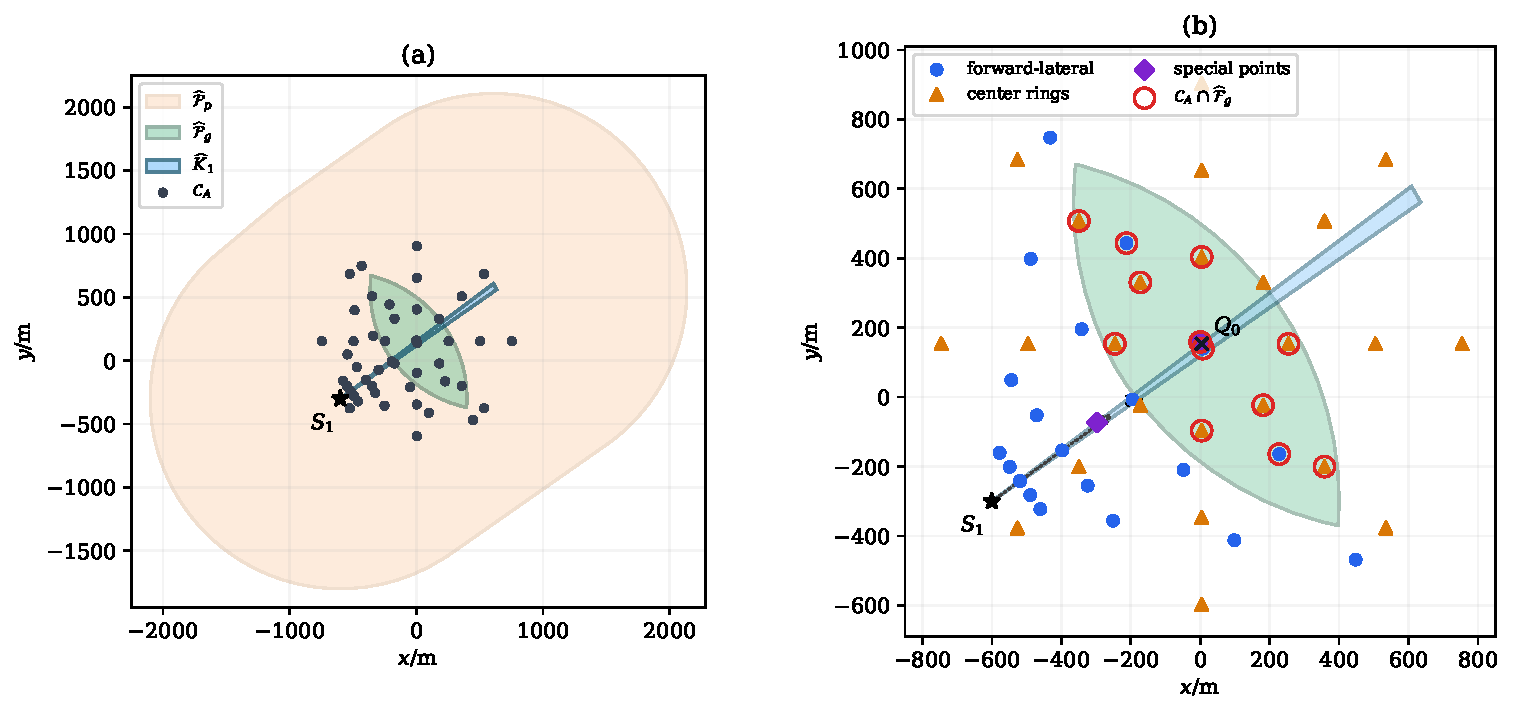
\includegraphics[width=0.94\textwidth]{figures/q2-discrete-candidates.pdf}
  \caption{候选区域内有限离散候选点的构造与筛选示意图}
  \label{fig:q2-discrete-candidates}
\end{figure}

对有限离散候选集 $\mathcal C_A$ 中的每个候选点，为同时衡量行动时间和定位不确定性，定义综合评分
\begin{equation}
  J(s)=T(s)+\lambda_RR_{\mathrm{wc}}(s),
  \qquad \lambda_R=0.5\ \mathrm{s/m}.
  \label{eq:q2-discrete-score}
\end{equation}

$\lambda_R$ 是平衡行动时间与定位不确定性半径的权重超参数，单位为 $\mathrm{s/m}$；本文取 $0.5\ \mathrm{s/m}$，其数值可按两项目标的相对偏好调整，并非题设常数。若 $\mathcal C_A^g$ 非空，则方案一选出的候选点为
\begin{equation}
  s_A=\operatorname*{arg\,min}_{s\in
  \mathcal C_A^g}J(s).
  \label{eq:q2-baseline-choice}
\end{equation}

若 $\mathcal C_A^g$ 为空，则退回全部 $\mathcal C_A$ 中求 $J(s)$ 最小的点，并通过式~\eqref{eq:q2-worst-radius} 中的无信号分支惩罚接收风险。该方案的最优性仅针对当前有限离散候选集、有限源场景和式~\eqref{eq:q2-discrete-score} 的综合评分成立。

\subsubsection{方案二：保证候选区域内的连续 Fisher 信息选点策略}

方案二是在保证接收候选区域 $\widehat{\mathcal F}_g$ 内连续改变测点坐标并产生候选点的策略。有限离散候选可能遗漏相邻点之间交会几何更好的位置，因此以 Fisher 信息矩阵衡量局部方位观测对源位置的辨识能力~\cite{fisher1922}。对检测点 $S_i=(x_i,y_i)$ 和源位置 $X=(x,y)$，理想方位观测为
\begin{equation}
  h_i(X)=\operatorname{atan2}(y-y_i,x-x_i),
\end{equation}

其中 $\operatorname{atan2}$ 为四象限反正切函数，示向度统一转换至 $[0,2\pi)$。

其对 $X$ 的梯度为
\begin{equation}
  q_i(X)=\nabla_X h_i(X)
  =\frac{1}{d_i^2}
  \begin{bmatrix}
    -(y-y_i)\\ x-x_i
  \end{bmatrix},
  \qquad d_i=\|X-S_i\|_2.
\end{equation}

为构造信息量替代目标，暂将两次角度扰动视为相互独立且具有相同局部方差 $\sigma_\theta^2$，则
\begin{equation}
  \mathcal I(s;X)
  =\frac{1}{\sigma_\theta^2}
  \left(q_1q_1^{\mathsf T}+q_2q_2^{\mathsf T}\right),
  \qquad S_2=s.
  \label{eq:q2-fim}
\end{equation}

设从两个检测点指向源的视线夹角为 $\phi(s;X)$。利用二维恒等式 $\det(aa^{\mathsf T}+bb^{\mathsf T})=(a_1b_2-a_2b_1)^2$，由式~\eqref{eq:q2-fim} 直接得
\begin{equation}
  \det\mathcal I(s;X)
  =\frac{\sin^2\phi(s;X)}
  {\sigma_\theta^4d_1^2d_2^2}.
  \label{eq:q2-fim-determinant}
\end{equation}

式~\eqref{eq:q2-fim-determinant} 表明，两条视线近似平行时，两次示向度提供的方向约束近似重复，交会定位结果对角度误差较为敏感；在距离相当时，较大的交会角通常提供更多定位信息；而观测距离过大会放大角度误差所导致的定位不确定性。

略去对所有候选点相同的 $\sigma_\theta^{-4}$，引入仅用于调整数值尺度的常数 $\kappa=10^{12}$，并用行动时间归一化，定义
\begin{equation}
  \Phi(s;X)=
  \frac{\kappa\sin^2\phi(s;X)}
  {d_1^2d_2^2T(s)}.
\end{equation}

当 $d_2\leq5\ \mathrm{m}$ 时，检测将进入近距离分支，不再适用常规示向度 Fisher 指标，因而在数值搜索中使用有界的有利近似 $\Phi(s;X)=\kappa/(25d_1^2T(s))$。又因首次检测已获得有效示向度，Fisher 场景构造时排除 $d_1\leq5\ \mathrm{m}$ 的退化点。
对 $\widehat K_1$ 每条边上的若干等分点及区域中心构造确定性场景集 $\mathcal S_F$，再取
\begin{equation}
  \Phi_{\mathrm{rob}}(s)
  =\min_{X\in\mathcal S_F}\Phi(s;X),
  \label{eq:q2-robust-fim}
\end{equation}

表示当前所检查源位置中的最小单位时间信息量。

记方案一选点的行动时间为 $T_A=T(s_A)$。为同时考察“较快到达”与“允许走得更远以改善交会几何”的情形，额外给出三档行动时间余量 $b\in\{15,30,60\}\ \mathrm{s}$，分别求解
\begin{equation}
  s_F^{(b)}
  =\operatorname*{arg\,max}_{s\in\widehat{\mathcal F}_g}
  \Phi_{\mathrm{rob}}(s),
  \qquad T(s)\leq T_A+b.
  \label{eq:q2-fim-budget}
\end{equation}

每档最多产生一个候选点，共同反映额外行动时间与交会几何之间的权衡。

求解时从保证域中心、边界顶点、边中点及离散候选中选取多个初始点，在 $16$ 个方向上进行投影模式搜索。试探点越出 $\widehat{\mathcal F}_g$ 时将其投影回可行多边形；若没有找到更优点，则将步长减半，直至步长由 $200\ \mathrm{m}$ 缩小至 $2\ \mathrm{m}$，或达到迭代次数、求解时间等预设上限；达到上限时返回已经搜索到的最优可行点。
\subsubsection{统一评价与最终选点}

方案一的 $J(s)$ 与方案二的 $\Phi_{\mathrm{rob}}(s)$ 量纲和物理含义均不同，不能直接根据两个数值判断测点优劣。因此，Fisher 信息优化只用于在保证接收区域内搜索可能具有较好交会几何的连续测点坐标，并不直接决定最终测点。三档预算所得候选均重新使用式~\eqref{eq:q2-worst-radius} 和式~\eqref{eq:q2-action-time} 计算
\begin{equation}
  \bigl(R_{\mathrm{wc}}(s),T(s),J(s)\bigr).
\end{equation}

在实际执行时，首先保留满足 $T(s)\leq T_A+30\ \mathrm{s}$ 的连续候选。$60\ \mathrm{s}$ 档产生的候选仅在其实际行动时间不超过 $T_A+30\ \mathrm{s}$ 时纳入最终可执行集。对每个保留的连续候选点，定义有序评价向量
\begin{equation}
  \boldsymbol z(s)=\left(R_{\mathrm{wc}}(s),T(s),
  -\Phi_{\mathrm{rob}}(s),s_x,s_y\right).
\end{equation}

按 $\boldsymbol z(s)$ 从左到右逐级比较：优先选择 $R_{\mathrm{wc}}$ 小的点，相同时比较行动时间，再比较信息量和坐标，得到连续代表点 $s_F$。

另在离散选点与三档连续候选组成的集合 $\mathcal C$ 中，保留时间与定位半径均不被其他点同时改善的非支配候选，供两目标权衡分析；最终执行仍按下述规则决定。

最终执行点只在方案一选点 $s_A$ 和连续代表点 $s_F$ 之间，按照“定位不确定性半径的最坏预测值优先、行动时间次之”的规则选取
\begin{equation}
  s^*=\operatorname*{lex\,arg\,min}_{s\in\{s_A,s_F\}}
  \left(R_{\mathrm{wc}}(s),T(s),s_x,s_y\right).
  \label{eq:q2-final-choice}
\end{equation}

其中 $\mathrm{lex}$ 表示上述逐级比较顺序，坐标仅用于消除并列结果。若连续优化不可用，则令 $s^*=s_A$。

\subsubsection{候选区域、选点策略总结及推广}

综上，实际候选区域为保证接收内近似 $\widehat{\mathcal F}_g$，推荐点由离散与连续方案统一复评分后按式~\eqref{eq:q2-final-choice} 选出。离散保证候选为空时回退至全部离散候选，并计入无信号风险；连续方案仅在保证域非空时运行。

这一策略可由“已有一个检测点”直接推广至“已有多个检测点”：用全部有效示向度约束更新当前区域 $\widehat K_n$，再以 $\widehat K_n$ 重新构造候选区域并选择第 $n+1$ 个检测点。问题三直接利用该递推方法实现全向干扰源的连续定位；问题四保留多观测区域更新和定位不确定性评价，但由于定向干扰源在距离足够近时仍可能因辐射方向不符而无信号，需将下一检测点扩展为从多个方向接近的探测点。
